\section{Introduction}
\label{sec:introduction}


The main objective of this laboratory assignment is to analyse a RC circuit in order to determine the natural and the forced responses and also a frequency analysis. The circuit under analysis is shown in Figure ~\ref{fig:circuit}.

In the next section (~\ref{sec:analysis}), we briefly explain the procedure to analyse the given circuit in six different subsections, each one to answer the different topics asked by the teacher. In order to solve the necessary calculations and obtain the values we used Octave maths tool. In this section, we also plotted graphics eand tables to a better analysis of the results.

Then, we resorted to Ngspice to simulate our circuit and obtain the simulated values for the same physical quantities previously calculated. These values will be shown in Section~\ref{sec:simulation}, divided by six subsections, five of which to explain in a more proper way what we simulated, and the last one to compare both theoretical and simulated results and give certain notes related to our analysis.

The report finishes with its conclusion, in section~\ref{sec:conclusion}, where we resume the most important topics of the lab assignment.

\begin{figure}[h] \centering
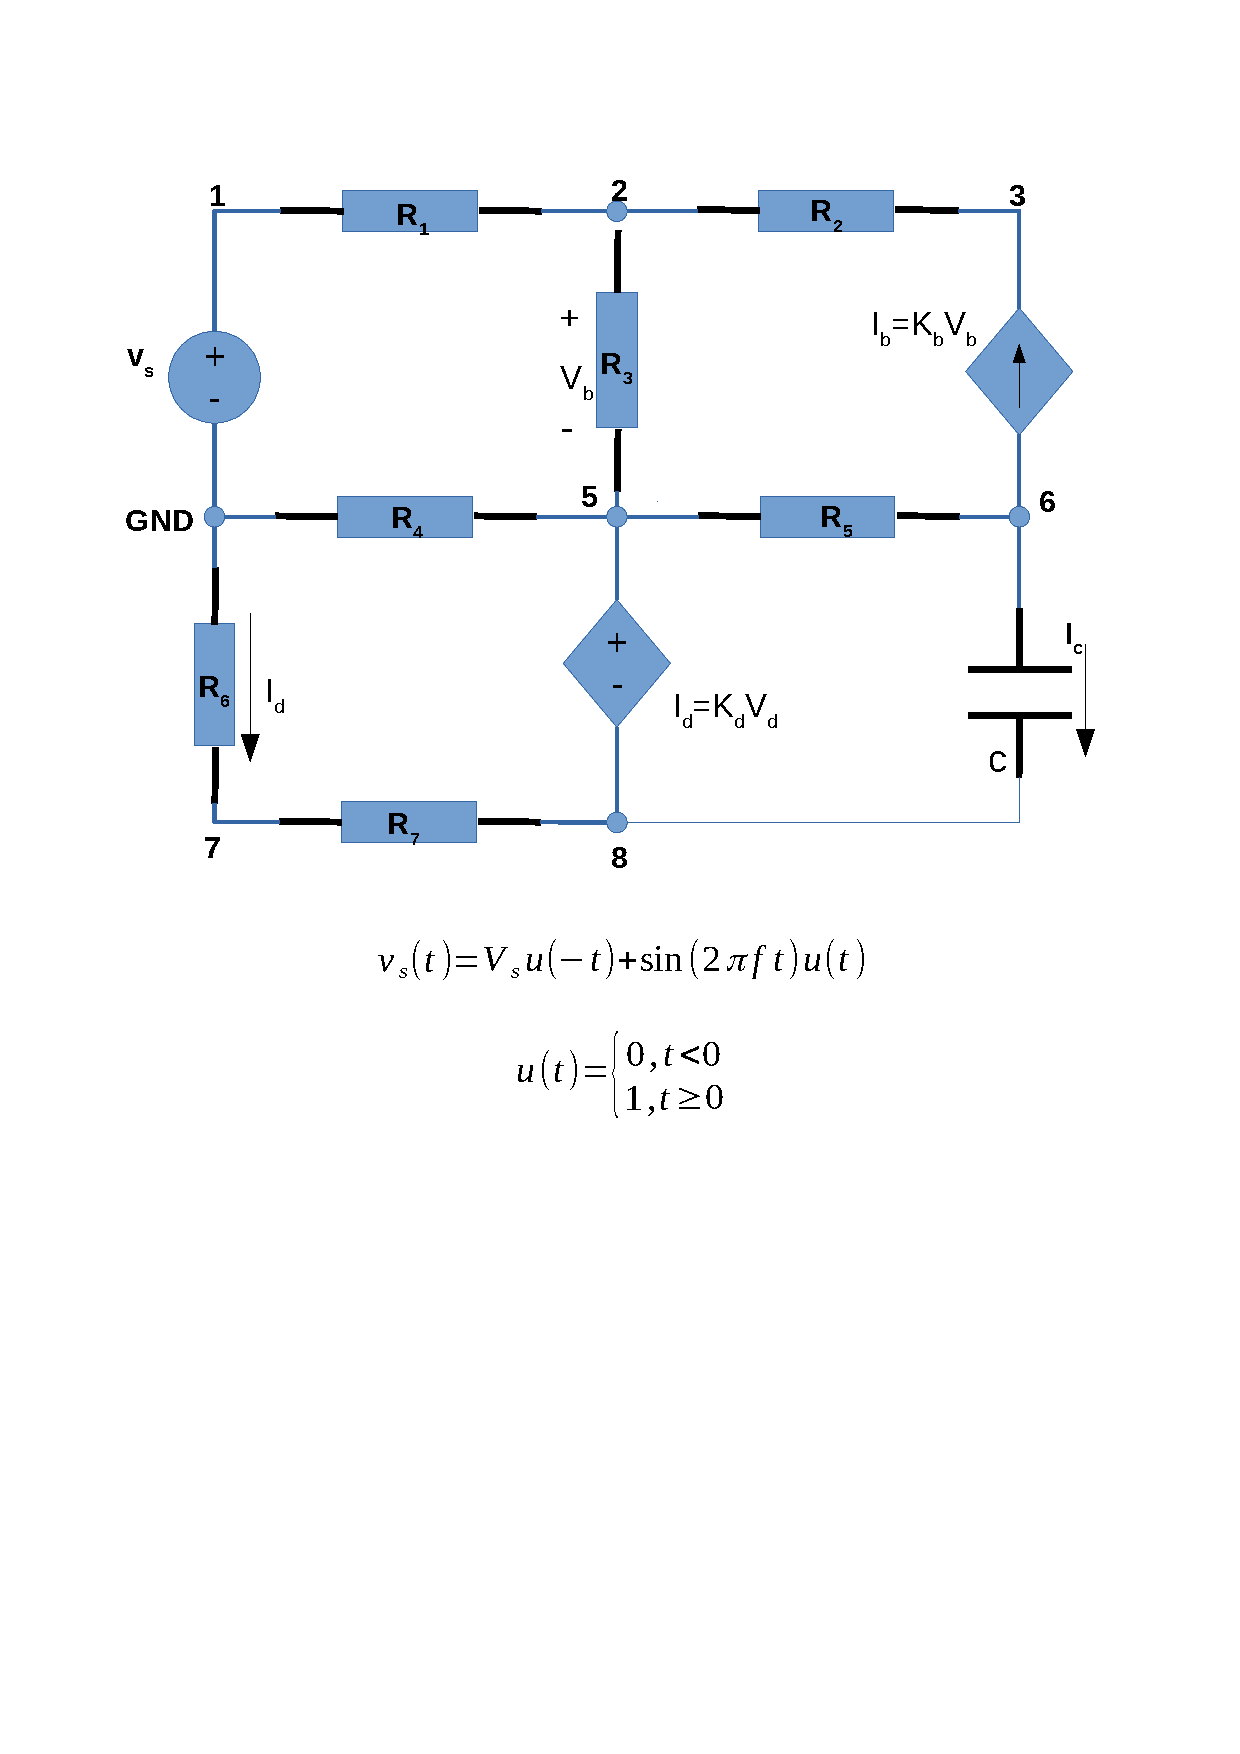
\includegraphics[width=0.6\linewidth]{circuit.pdf}
\caption{Circuit under analysis.}
\label{fig:circuit}
\end{figure}

